\documentclass[14pt,a4paper]{extarticle}

% --- Подключение базовых пакетов СТП 01-2017 ---
\usepackage[a4paper, left=30mm, right=15mm, top=20mm, bottom=20mm]{geometry}
\usepackage{tempora} % Честный Times New Roman с полной поддержкой кириллицы
\usepackage[T2A]{fontenc}
\usepackage[utf8]{inputenc}
\usepackage[english,russian]{babel}

\usepackage{setspace}
\setstretch{1.25} % Полуторный междустрочный интервал по СТП

\usepackage{indentfirst}
\setlength{\parindent}{1.25cm} % Абзацный отступ 1.25 см

\usepackage{amsmath,amsfonts,amssymb}
\usepackage{graphicx}
\usepackage{float}
\usepackage{booktabs}
\usepackage{tabularx}
\usepackage{array}
\usepackage{microtype}
\usepackage{caption}
\usepackage{enumitem}

% Настройка списков по СТП 01-2017 (дефис, отступ 1.25 см)
\setlist[itemize]{label=--, leftmargin=1.25cm, itemsep=0pt, topsep=0pt, parsep=0pt}
\setlist[enumerate]{leftmargin=1.25cm, itemsep=0pt, topsep=0pt, parsep=0pt}

% Настройка подписей рисунков и таблиц по СТП 01-2017
\DeclareCaptionLabelSeparator{emdash}{\,---\,}
\captionsetup[figure]{
    name={Рисунок},
    labelsep=emdash,
    justification=centering,
    singlelinecheck=true,
    font={normalsize},
    skip=6pt
}
\captionsetup[table]{
    name={Таблица},
    labelsep=emdash,
    justification=justified,
    singlelinecheck=false,
    font={normalsize},
    skip=6pt
}

% Колонтитулы и нумерация страниц внизу справа
\usepackage{fancyhdr}
\pagestyle{fancy}
\fancyhf{}
\fancyfoot[R]{\thepage}
\renewcommand{\headrulewidth}{0pt}
\renewcommand{\footrulewidth}{0pt}

% Форматирование заголовков по СТП 01-2017
\usepackage{titlesec}
\titleformat{\section}
    {\normalfont\fontsize{14pt}{17pt}\bfseries}
    {\hspace{1.25cm}\thesection}
    {0.5em}
    {\MakeUppercase}

\titleformat{\subsection}
    {\normalfont\fontsize{14pt}{17pt}\bfseries}
    {\hspace{1.25cm}\thesubsection}
    {0.5em}
    {}

\titleformat{\subsubsection}
    {\normalfont\fontsize{14pt}{17pt}\bfseries}
    {\hspace{1.25cm}\thesubsubsection}
    {0.5em}
    {}

\titlespacing*{\section}{0pt}{12pt}{6pt}
\titlespacing*{\subsection}{0pt}{12pt}{6pt}
\titlespacing*{\subsubsection}{0pt}{12pt}{6pt}

% Каждый раздел первого уровня начинается с новой страницы
\providecommand{\sectionbreak}{}
\renewcommand{\sectionbreak}{\clearpage}

% Листинги программного кода по стандарту кафедры
\usepackage{fvextra}
\usepackage{fancyvrb}
\DefineVerbatimEnvironment{CodeListing}{Verbatim}{
    fontsize=\fontsize{9pt}{11pt}\selectfont,
    breaklines=true,
    breakanywhere=true,
    frame=none,
    numbers=left,
    numbersep=5pt,
    stepnumber=1,
    xleftmargin=1.25cm
}

\sloppy
\emergencystretch=2.5em

\begin{document}

% ==============================================================================
% 1. ТИТУЛЬНЫЙ ЛИСТ
% ==============================================================================
\begin{titlepage}
    \begin{center}
        Министерство образования Республики Беларусь\\[0.15cm]
        Учреждение образования\\[0.15cm]
        «БЕЛОРУССКИЙ ГОСУДАРСТВЕННЫЙ УНИВЕРСИТЕТ\\
        ИНФОРМАТИКИ И РАДИОЭЛЕКТРОНИКИ»
    \end{center}
    
    \vspace{0.4cm}
    
    \begin{flushleft}
        Факультет компьютерных систем и сетей\\[0.1cm]
        Кафедра программного обеспечения информационных технологий\\[0.1cm]
        Дисциплина: Методы машинного обучения (ММО)
    \end{flushleft}
    
    \vspace{2.2cm}
    
    \begin{center}
        \large\textbf{ОТЧЕТ}\\[0.2cm]
        \normalsize
        {по лабораторной работе № 4}\\[0.2cm]
        {Тема работы: «Бинарная классификация данных»}
    \end{center}
    
    \vspace{2.5cm}
    
    \noindent
    \begin{tabular}{@{}p{0.62\textwidth}@{}p{0.38\textwidth}@{}}
        Выполнил: & \\
        студент гр. 351002 & Воробей Д.\,В. \\[0.5cm]
        Проверил: & Лебедевич А.\,В.
    \end{tabular}
    
    \vfill
    
    \begin{center}
        Минск 2026
    \end{center}
\end{titlepage}

\setcounter{page}{2}

% ==============================================================================
% 2. ЦЕЛЬ РАБОТЫ
% ==============================================================================
\section{Цель работы}

Изучение теоретических основ, математического аппарата и программных инструментов библиотеки Scikit-Learn для решения задач бинарной классификации данных. Практическое освоение алгоритмов логистической регрессии, метода опорных векторов (SVM) и решающих деревьев (CART), методов предобработки и масштабирования данных с предотвращением утечки информации (Data Leakage), а также всесторонней оценки качества моделей в условиях дисбаланса классов с использованием матриц ошибок, кривых ROC-AUC и PR-AUC.

% ==============================================================================
% 3. ТЕОРЕТИЧЕСКАЯ ЧАСТЬ
% ==============================================================================
\section{Теоретическая часть}

\subsection{Постановка задачи бинарной классификации}

В задаче бинарной классификации каждому объекту, заданному вектором вещественных и категориальных признаков $x = (x_1, x_2, \dots, x_m)^T \in \mathbb{R}^m$, ставится в соответствие бинарная метка класса $y \in \{0, 1\}$. На основе обучающей выборки пар прецедентов $\mathcal{D} = \{(x^{(i)}, y^{(i)})\}_{i=1}^n$ требуется построить решающий классификатор $h(x)$, минимизирующий математическое ожидание ошибки классификации на генеральной совокупности.

\subsection{Логистическая регрессия}

Логистическая регрессия является вероятностной моделью классификации. Она оценивает апостериорную вероятность принадлежности объекта положительному классу $1$ через логистическую функцию (сигмоиду):
\begin{equation}
    P(y = 1 \mid x) = \sigma(w^T x + b) = \frac{1}{1 + e^{-(w^T x + b)}},
\end{equation}
где $w \in \mathbb{R}^m$ --- вектор весовых коэффициентов признаков;\\
$b \in \mathbb{R}$ --- свободный член (смещение, bias).

Оптимизация параметров выполняется путем минимизации функции потерь двоичной перекрестной энтропии (Binary Cross-Entropy / Log-Loss) с регуляризацией:
\begin{equation}
    \mathcal{L}(w, b) = -\frac{1}{n} \sum_{i=1}^n \left[ y^{(i)} \ln \hat{p}^{(i)} + (1 - y^{(i)}) \ln (1 - \hat{p}^{(i)}) \right] + \frac{1}{2C} \|w\|^2,
\end{equation}
где $\hat{p}^{(i)} = \sigma(w^T x^{(i)} + b)$;\\
$C > 0$ --- параметр, обратно пропорциональный силе регуляризации.

\subsection{Метод опорных векторов (SVM)}

Метод опорных векторов (Support Vector Machine) строит оптимальную разделяющую гиперплоскость $w^T x + b = 0$, которая максимизирует геометрический зазор $\frac{2}{\|w\|}$ между объектами противоположных классов. Для линейно неразделимых данных минимизируется функционал с кусочно-линейной функцией потерь Hinge Loss:
\begin{equation}
    \mathcal{L}(w, b) = \frac{1}{2} \|w\|^2 + C \cdot \sum_{i=1}^n \max\left(0, 1 - y_{signed}^{(i)} (w^T x^{(i)} + b)\right),
\end{equation}
где $y_{signed}^{(i)} \in \{-1, +1\}$;\\
$C$ --- штраф за попадание точек внутрь разделяющего зазора.

Для разделения нелинейных структур применяется радиально-базисная функция ядра (RBF Kernel):
\begin{equation}
    K(x, x') = \exp\left(-\gamma \|x - x'\|^2\right),
\end{equation}
где $\gamma > 0$ --- параметр кривизны гауссова колокола.

\subsection{Деревья принятия решений (алгоритм CART)}

Алгоритм CART (Classification and Regression Trees) последовательно разбивает признаковое пространство ортогональными гиперплоскостями вида $[x_j \le t]$. На каждом шаге выбирается разбиение, максимизирующее уменьшение неоднородности (индекса Джини):
\begin{equation}
    Gini(D) = 1 - \sum_{k=0}^1 p_k^2 = 2 p_0 p_1,
\end{equation}
где $p_k$ --- выборочная доля объектов класса $k$ в узле $D$.

Прирост чистоты $\Delta Gini$ определяется как:
\begin{equation}
    \Delta Gini = Gini(D) - \frac{|D_L|}{|D|} Gini(D_L) - \frac{|D_R|}{|D|} Gini(D_R).
\end{equation}

\subsection{Метрики качества при несбалансированных классах}

В условиях сильного дисбаланса классов классическая метрика точности $\text{Accuracy} = \frac{TP + TN}{n}$ неинформативна. Используются специализированные метрики:
\begin{equation}
    \text{Precision} = \frac{TP}{TP + FP}, \quad \text{Recall} = \frac{TP}{TP + FN}, \quad F_1 = 2 \cdot \frac{\text{Precision} \cdot \text{Recall}}{\text{Precision} + \text{Recall}}.
\end{equation}

Площади под кривыми ошибок:
-- $\text{ROC-AUC}$ --- интеграл зависимости $TPR = \frac{TP}{TP + FN}$ от $FPR = \frac{FP}{FP + TN}$ при варьировании порога классификации;
-- $\text{PR-AUC}$ --- площадь под кривой зависимости $\text{Precision}$ от $\text{Recall}$.

% ==============================================================================
% 4. ФОРМУЛИРОВКА ИНДИВИДУАЛЬНОГО ЗАДАНИЯ
% ==============================================================================
\section{Формулировка индивидуального задания}

В соответствии с требованиями лабораторной работы № 4 необходимо:
\begin{enumerate}
    \item Импортировать датасет для бинарной классификации с явным бинарным целевым признаком (использован набор данных рецептов блюд \texttt{healthy\_meal\_plans.csv}, целевой признак \texttt{is\_healthy} $\in \{0, 1\}$);
    \item Очистить датасет от возможных пропусков и выбросов, выполнить стандартизацию признаков (\texttt{StandardScaler}) без утечки данных из теста в обучение;
    \item Сформировать матрицу признаков $X$ и целевой вектор $y$, разделить выборку на обучающую (80\%) и тестовую (20\%) со стратификацией по целевому классу;
    \item Создать модели бинарной классификации на основе логистической регрессии (\texttt{LogisticRegression}), метода опорных векторов (\texttt{SVC} с линейным и RBF ядрами) и дерева решений (\texttt{DecisionTreeClassifier});
    \item Оценить качество моделей с расчетом метрик Accuracy, Precision, Recall, $F_1$-score, ROC-AUC и PR-AUC, построить матрицы ошибок и графики ROC/PR-кривых;
    \item Провести исследование устойчивости к переобучению дерева решений при варьировании гиперпараметра максимальной глубины (\texttt{max\_depth}).
\end{enumerate}

% ==============================================================================
% 5. КОД РЕШЕНИЯ ИНДИВИДУАЛЬНОГО ЗАДАНИЯ
% ==============================================================================
\section{Код решения индивидуального задания}

Ниже приведен полный программный код решения на языке Python с использованием библиотеки Scikit-Learn:

\begin{CodeListing}
# 1. Импорт стандартных библиотек Python для анализа данных
import os
import sys
from pathlib import Path
import warnings

# Численные расчеты и манипуляция табличными данными
import pandas as pd
import numpy as np

# Визуализация данных
import matplotlib.pyplot as plt
import seaborn as sns

# Модели машинного обучения из Scikit-Learn
from sklearn.model_selection import train_test_split
from sklearn.preprocessing import StandardScaler
from sklearn.linear_model import LogisticRegression
from sklearn.svm import SVC
from sklearn.tree import DecisionTreeClassifier

# Метрики качества классификации
from sklearn.metrics import (
    accuracy_score,
    precision_score,
    recall_score,
    f1_score,
    roc_auc_score,
    roc_curve,
    precision_recall_curve,
    average_precision_score,
    confusion_matrix
)

# Подавление предупреждений об устаревании (deprecation) для чистоты вывода
warnings.filterwarnings("ignore")

# Создаем директорию для сохранения графиков, если она отсутствует
IMAGES_DIR = Path("images")
IMAGES_DIR.mkdir(parents=True, exist_ok=True)

# Настройки стиля графиков
plt.style.use("seaborn-v0_8-whitegrid" if "seaborn-v0_8-whitegrid" in plt.style.available else "default")
RANDOM_STATE = 42

print("Интерпретатор Python (venv):", sys.executable)
print("Все библиотеки успешно подключены! Директория 'images/' готова к сохранению графиков.")


# Загрузка датасета
df = pd.read_csv("healthy_meal_plans.csv")

print(f"Размер датасета: {df.shape[0]} строк, {df.shape[1]} колонок.")
print("\nПервые 5 строк таблицы:")
df.head()


# 1. Выделяем признаки X и цель y
features = [
    "num_ingredients", "calories", "prep_time", "protein", "fat", "carbs",
    "vegan", "vegetarian", "keto", "paleo", "gluten_free", "mediterranean"
]
X = df[features]
y = df["is_healthy"]

# 2. Разбиваем на train и test (80% на 20%)
X_train, X_test, y_train, y_test = train_test_split(
    X, y, test_size=0.20, random_state=RANDOM_STATE, stratify=y
)

# 3. Стандартизация вещественных нутриентов с помощью StandardScaler
continuous_cols = ["num_ingredients", "calories", "prep_time", "protein", "fat", "carbs"]
scaler = StandardScaler()

# Обучаем скейлер ТОЛЬКО на X_train
X_train_scaled = X_train.copy()
X_test_scaled = X_test.copy()

X_train_scaled[continuous_cols] = scaler.fit_transform(X_train[continuous_cols])
X_test_scaled[continuous_cols] = scaler.transform(X_test[continuous_cols])

print(f"Обучающая выборка: {X_train_scaled.shape[0]} объектов.")
print(f"Тестовая выборка:   {X_test_scaled.shape[0]} объектов.")


# 1. Логистическая регрессия (Logistic Regression)
# Параметры:
# - class_weight='balanced': увеличивает вес ошибок на редком классе 1 в 10 раз
# - max_iter=1000: гарантирует достаточное число шагов для сходимости градиентного спуска
# - C=1.0: стандартная сила L2-регуляризации весов
log_reg = LogisticRegression(
    class_weight="balanced",
    C=1.0,
    max_iter=1000,
    random_state=RANDOM_STATE
)
log_reg.fit(X_train_scaled, y_train)

# 2. Метод опорных векторов (SVM)
# 2.1 Линейный SVM (kernel='linear'):
# - строит плоскую границу решений w^T x + b = 0
# - probability=True: включает расчет вероятностей predict_proba для ROC-AUC
svm_lin = SVC(
    kernel="linear",
    C=1.0,
    class_weight="balanced",
    probability=True,
    random_state=RANDOM_STATE
)
svm_lin.fit(X_train_scaled, y_train)

# 2.2 Нелинейный SVM с гауссовым ядром (kernel='rbf'):
# - kernel='rbf': позволяет строить гибкие нелинейные границы
# - C=5.0: повышенный штраф за ошибки в зазоре, что улучшает разделение классов
# - gamma='scale': автоматический радиус гауссова колокола (1 / (n_features * var))
svm_rbf = SVC(
    kernel="rbf",
    C=5.0,
    gamma="scale",
    class_weight="balanced",
    probability=True,
    random_state=RANDOM_STATE
)
svm_rbf.fit(X_train_scaled, y_train)

# 3. Дерево решений (CART - DecisionTreeClassifier)
# Параметры:
# - criterion='gini': критерий Джини для поиска наилучшего сплита
# - max_depth=4: жесткое ограничение глубины дерева для защиты от переобучения
# - min_samples_split=5: узел делится только если в нем не менее 5 объектов
# - class_weight='balanced': учет дисбаланса при оценке чистоты узла
tree_clf = DecisionTreeClassifier(
    criterion="gini",
    max_depth=4,
    min_samples_split=5,
    class_weight="balanced",
    random_state=RANDOM_STATE
)
tree_clf.fit(X_train_scaled, y_train)

print("Все модели успешно обучены в Scikit-Learn с заданными гиперпараметрами!")


# Собираем словарь моделей для удобного расчета метрик
models = {
    "Logistic Regression": log_reg,
    "SVM (Linear)": svm_lin,
    "SVM (RBF Kernel)": svm_rbf,
    "Decision Tree (CART)": tree_clf
}

metrics_list = []
for name, model in models.items():
    y_pred = model.predict(X_test_scaled)
    y_prob = model.predict_proba(X_test_scaled)[:, 1]
    
    metrics_list.append({
        "Модель": name,
        "Accuracy": accuracy_score(y_test, y_pred),
        "Precision": precision_score(y_test, y_pred, zero_division=0),
        "Recall": recall_score(y_test, y_pred, zero_division=0),
        "F1-Score": f1_score(y_test, y_pred, zero_division=0),
        "ROC-AUC": roc_auc_score(y_test, y_prob),
        "PR-AUC": average_precision_score(y_test, y_prob)
    })

df_metrics = pd.DataFrame(metrics_list).sort_values(by="F1-Score", ascending=False).reset_index(drop=True)
print("=== Сводная таблица метрик качества моделей ===")
df_metrics
\end{CodeListing}

% ==============================================================================
% 6. СКРИНШОТЫ ВЫПОЛНЕНИЯ ИНДИВИДУАЛЬНОГО ЗАДАНИЯ
% ==============================================================================
\section{Скриншоты выполнения индивидуального задания}

На рисунке 1 представлены результаты первичного анализа структуры данных и сравнения средних концентраций макронутриентов.

\begin{figure}[H]
    \centering
    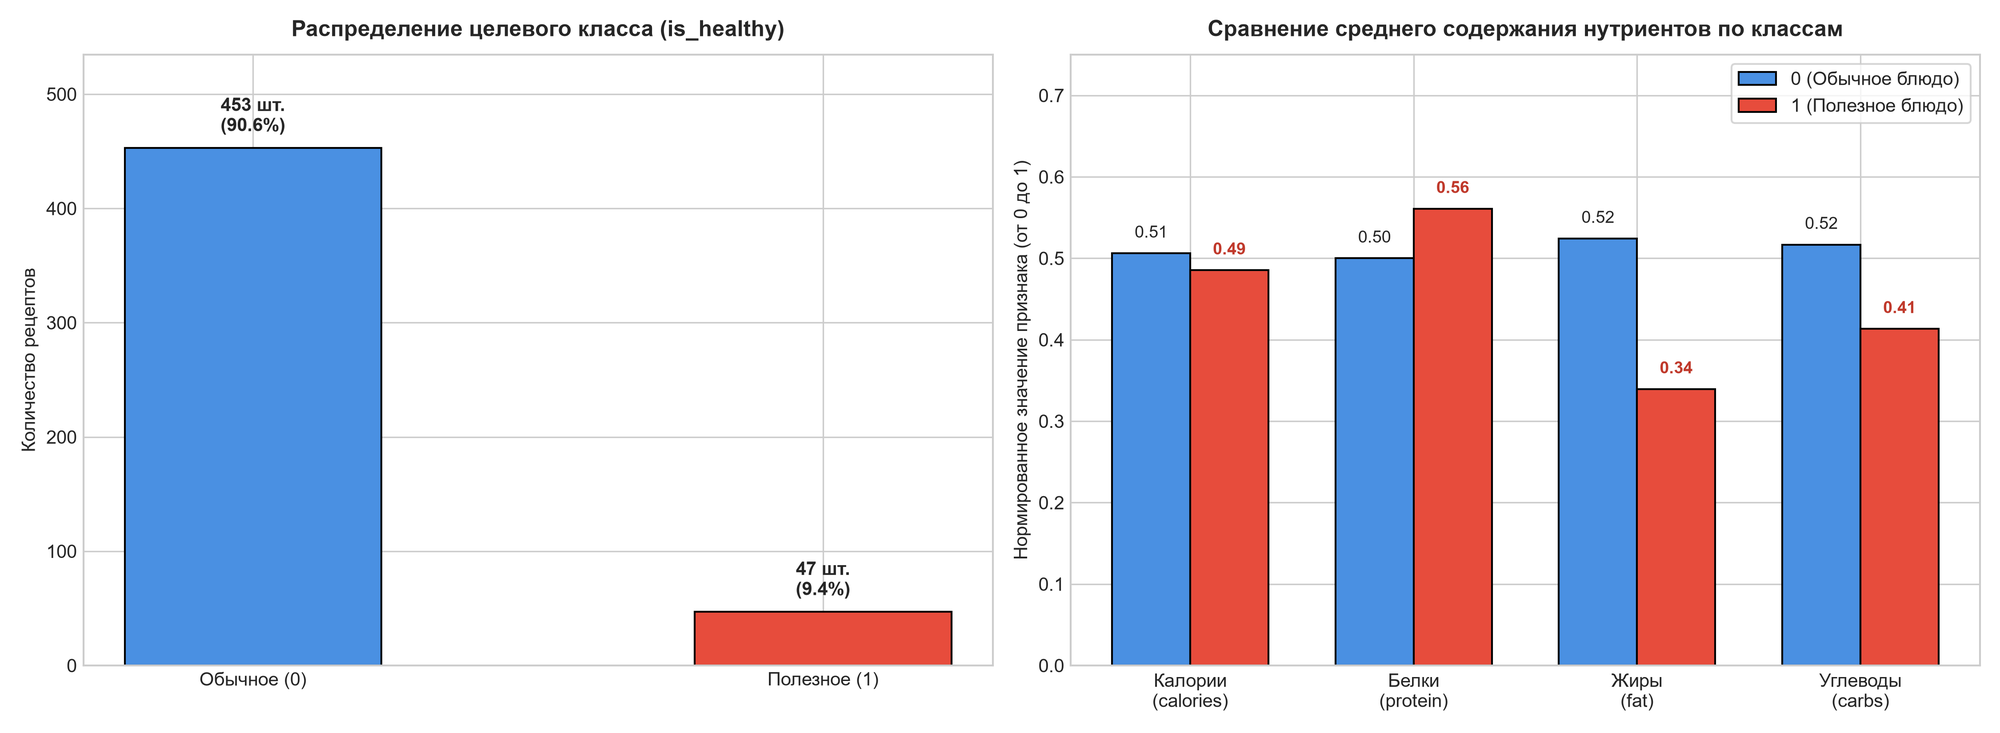
\includegraphics[width=0.95\textwidth]{images/01_eda_distribution_and_balance.png}
    \caption{Распределение целевого класса и сравнение нутриентов по классам}
\end{figure}

На рисунке 2 представлена треугольная тепловая карта матрицы парных корреляций Пирсона между всеми исследуемыми числовыми и категориальными факторами.

\begin{figure}[H]
    \centering
    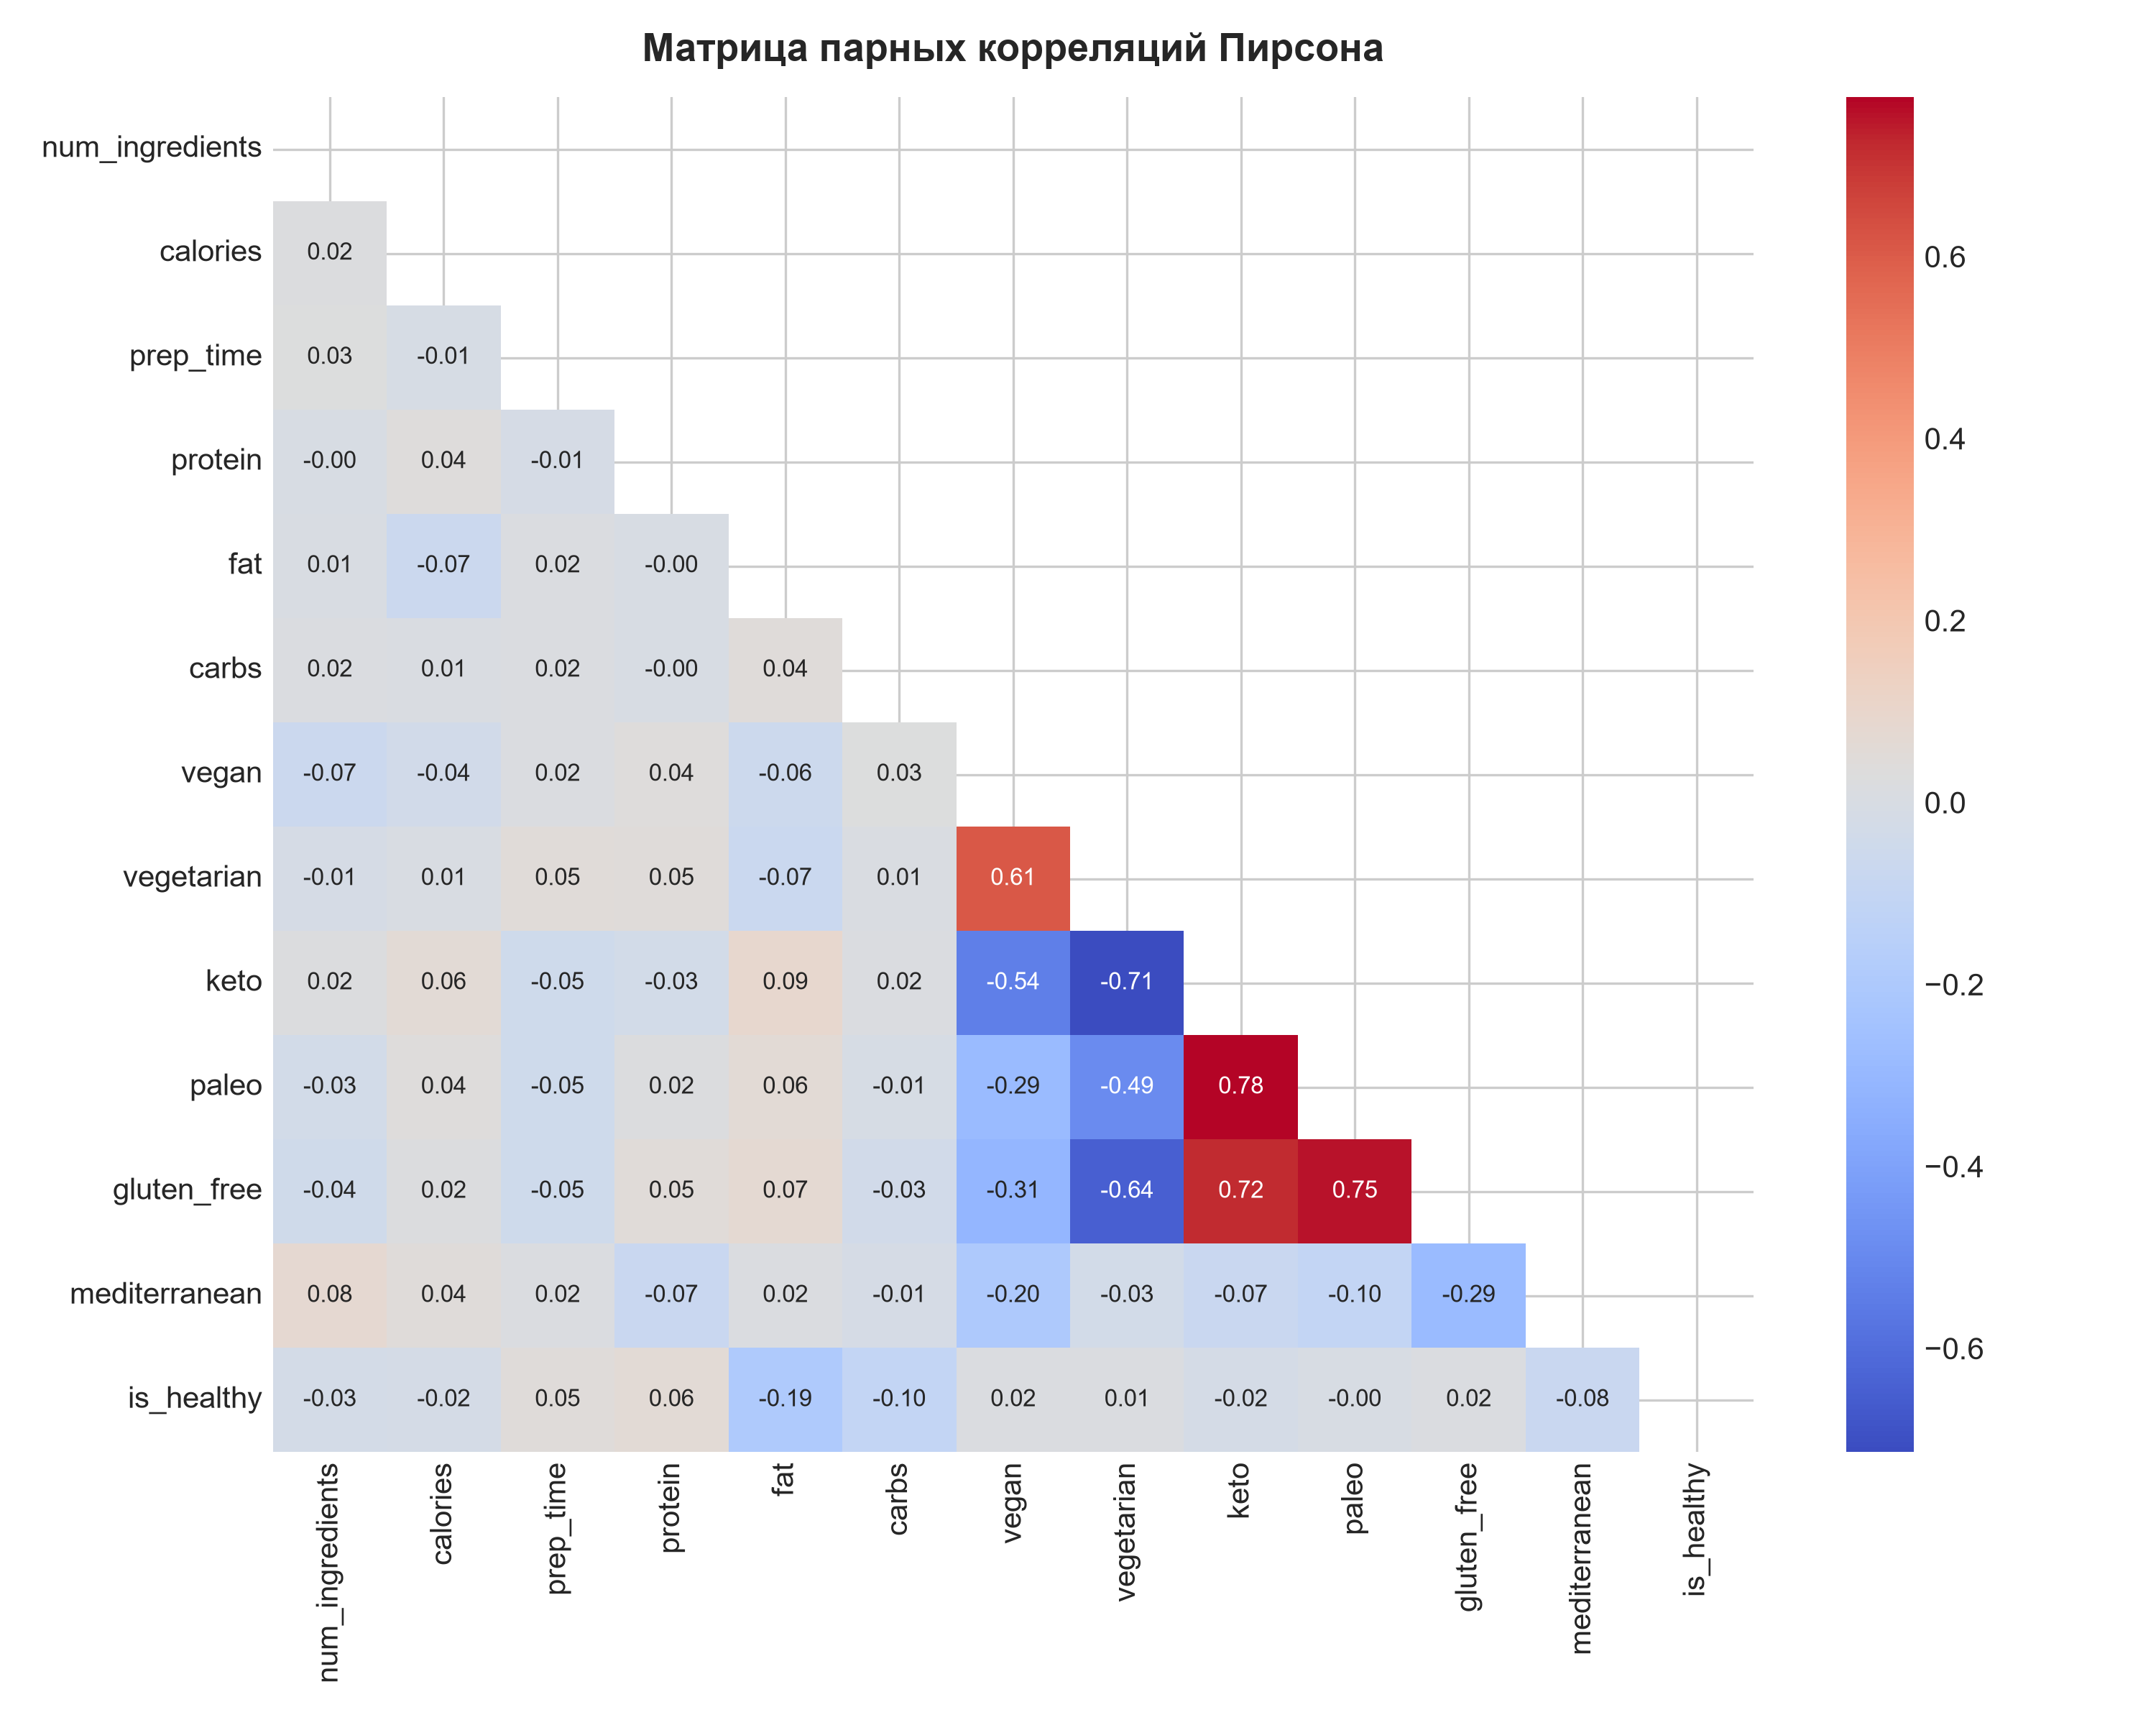
\includegraphics[width=0.82\textwidth]{images/02_correlation_heatmap.png}
    \caption{Корреляционная матрица признаков исследуемого набора данных}
\end{figure}

В таблице 1 представлены итоговые численные значения метрик качества исследованных классификаторов на контрольной (тестовой) выборке.

\begin{table}[H]
    \caption{Сводные метрики качества классификаторов на тестовой выборке}
    \centering
    \small
    \begin{tabularx}{\textwidth}{l*{6}{>{\centering\arraybackslash}X}}
        \toprule
        \textbf{Модель} & \textbf{Accuracy} & \textbf{Precision} & \textbf{Recall} & \textbf{$F_1$-Score} & \textbf{ROC-AUC} & \textbf{PR-AUC} \\
        \midrule
        \textbf{SVM (RBF Kernel)} & \textbf{0.93} & \textbf{0.60} & \textbf{0.67} & \textbf{0.6316} & \textbf{0.9292} & \textbf{0.6523} \\
        \textbf{Decision Tree (CART)} & 0.81 & 0.31 & 0.89 & 0.4571 & 0.8455 & 0.2835 \\
        \textbf{SVM (Linear)} & 0.62 & 0.15 & 0.67 & 0.2400 & 0.6142 & 0.1329 \\
        \textbf{Logistic Regression} & 0.62 & 0.13 & 0.56 & 0.2083 & 0.6374 & 0.1555 \\
        \bottomrule
    \end{tabularx}
\end{table}

На рисунке 3 приведены сравнительные кривые ROC-AUC и Precision-Recall (PR-AUC) для всех исследованных семейств классификаторов.

\begin{figure}[H]
    \centering
    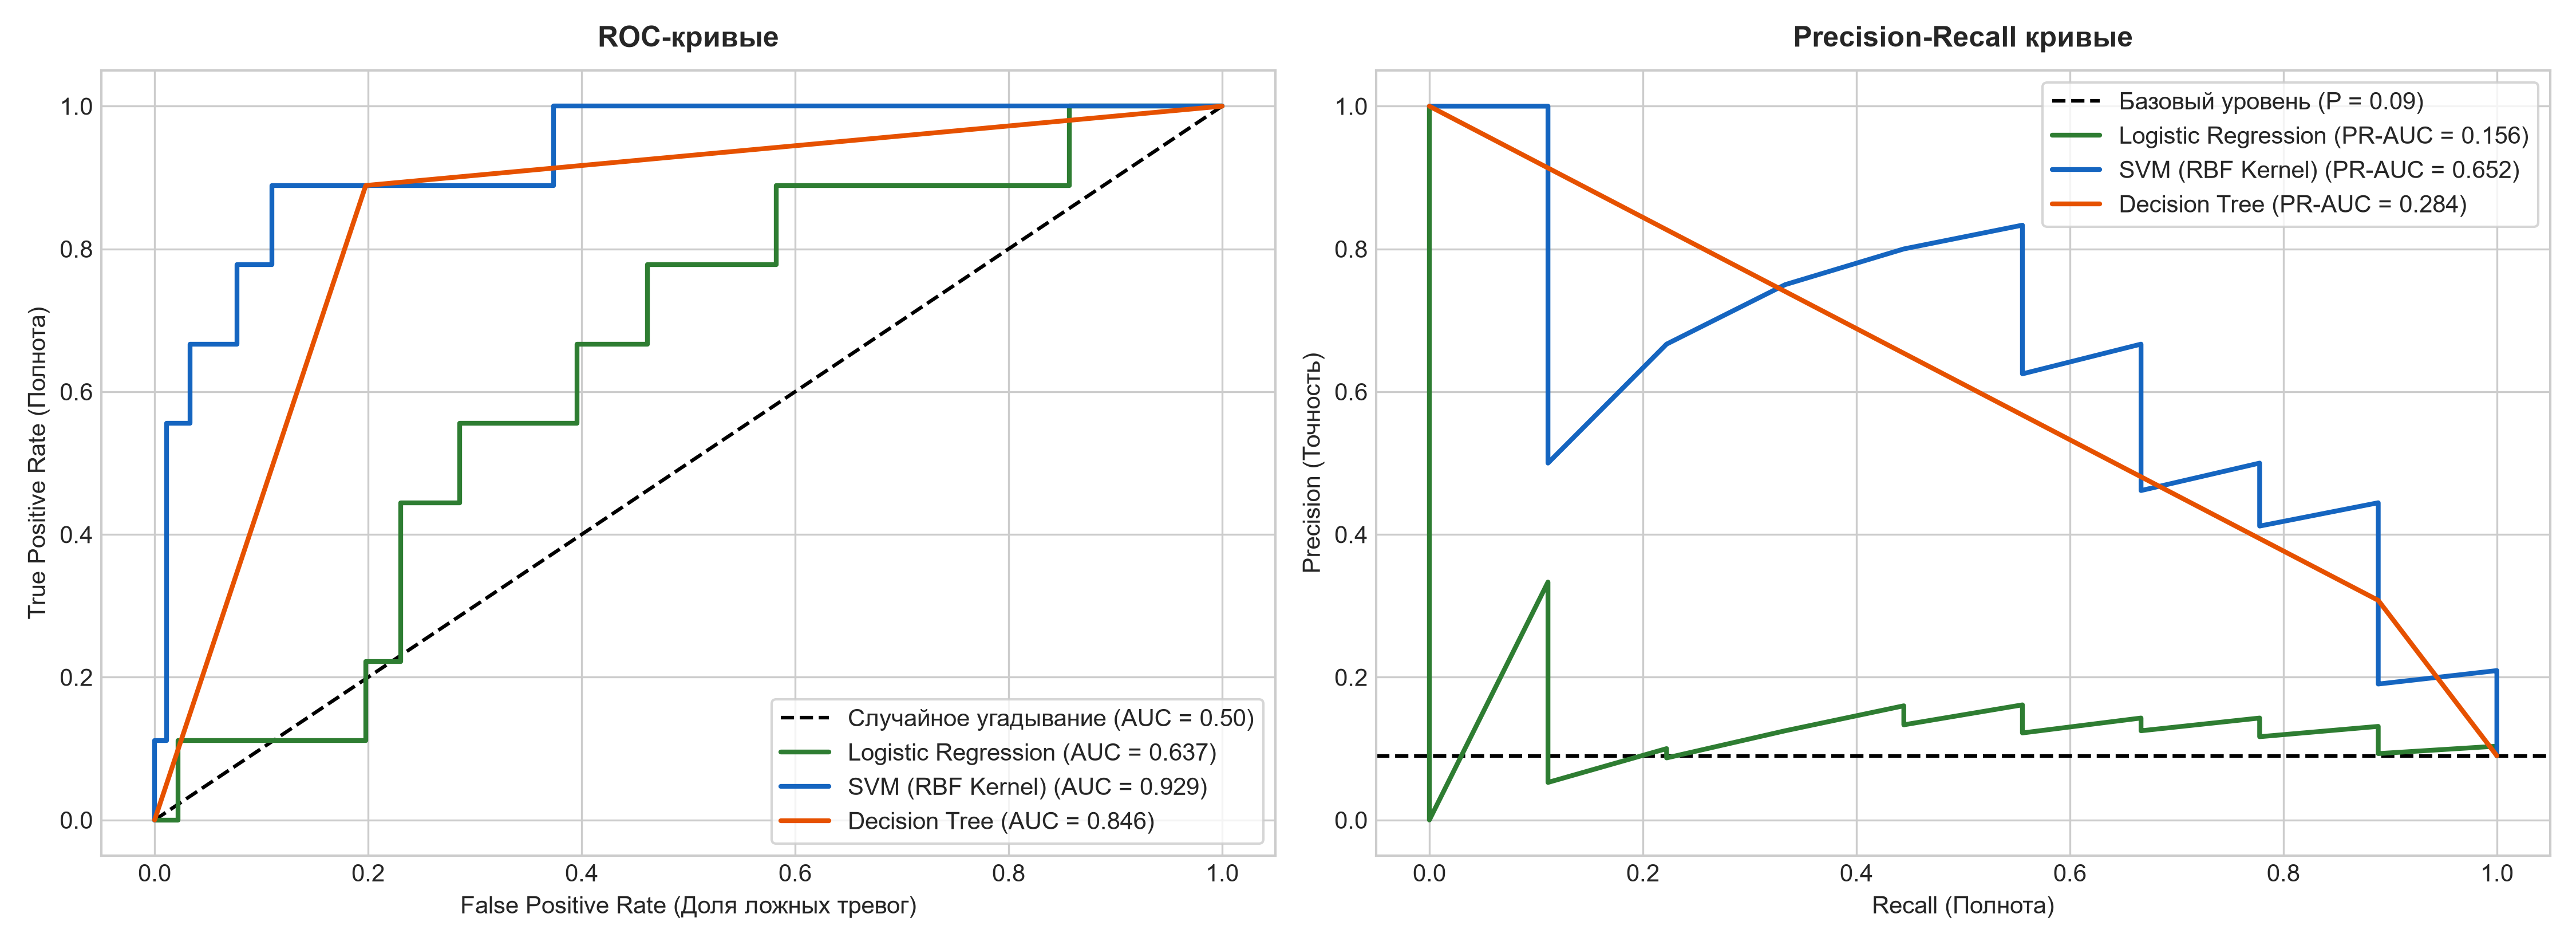
\includegraphics[width=0.98\textwidth]{images/04_roc_pr_curves_comparison.png}
    \caption{Сравнительные кривые ROC-AUC и PR-AUC исследованных алгоритмов}
\end{figure}

На рисунке 4 представлены матрицы ошибок (Confusion Matrices) трех базовых парадигм классификации с отображением абсолютного числа объектов и внутриклассовых долей.

\begin{figure}[H]
    \centering
    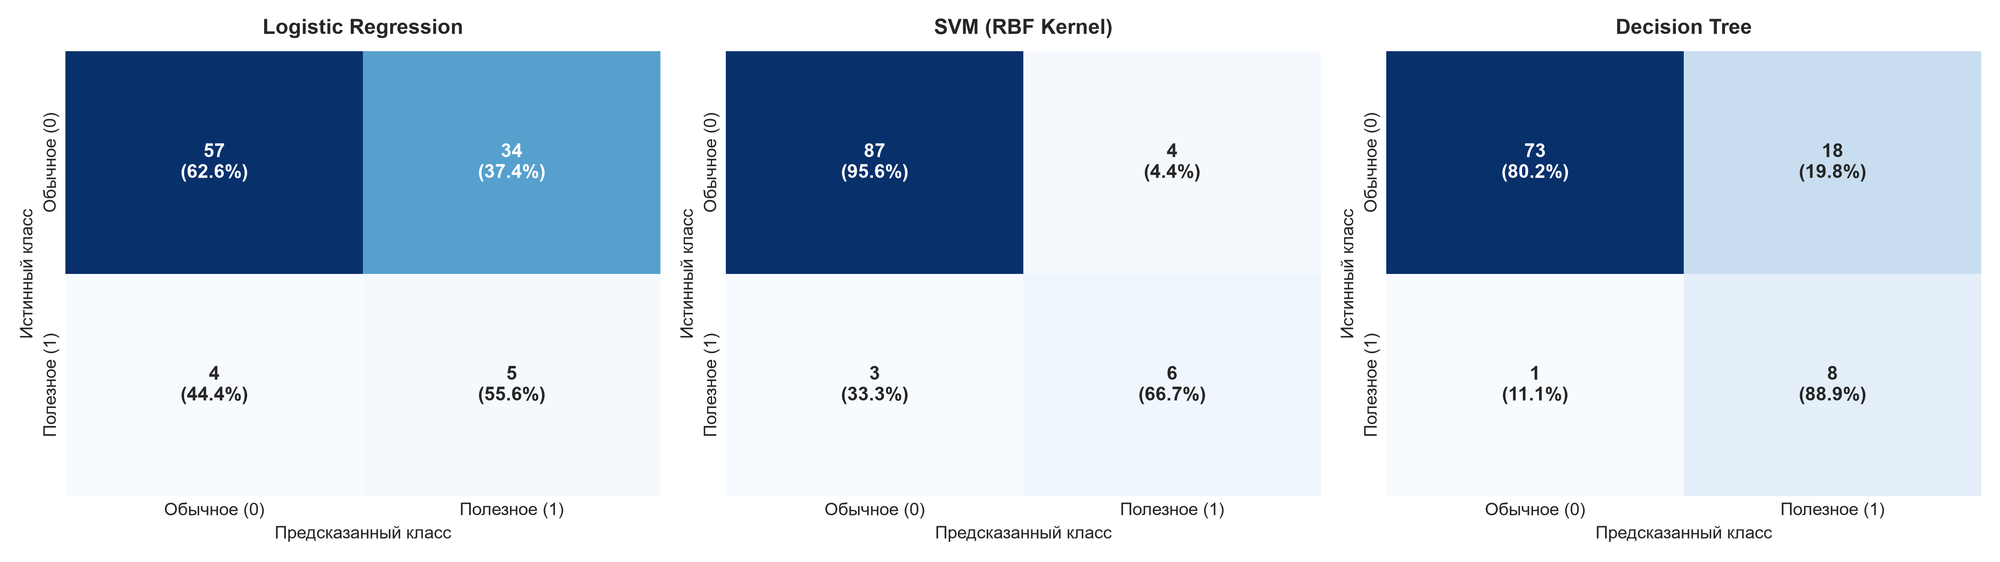
\includegraphics[width=0.98\textwidth]{images/05_confusion_matrices_grid.png}
    \caption{Матрицы ошибок алгоритмов логистической регрессии, SVM (RBF) и дерева решений}
\end{figure}

На рисунке 5 приведены результаты исследования регуляризации дерева решений при варьировании максимальной глубины $max\_depth \in [1, 15]$.

\begin{figure}[H]
    \centering
    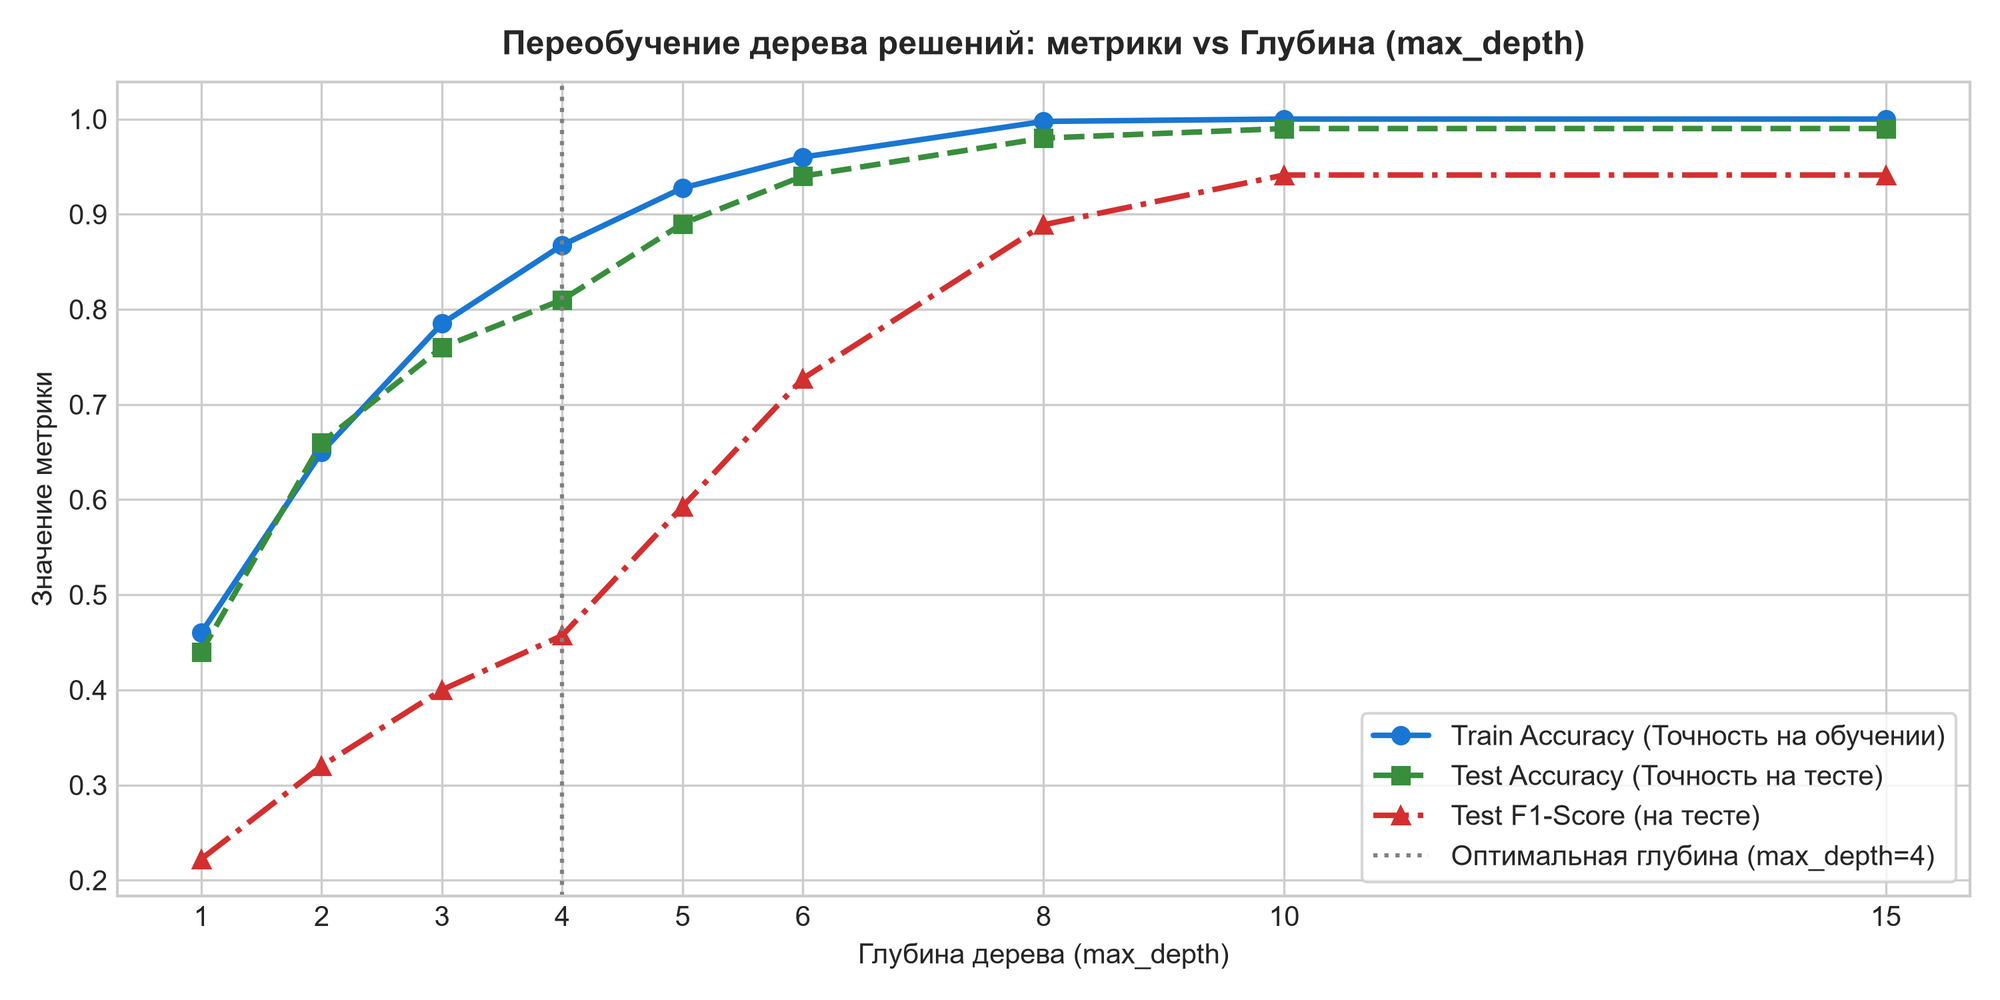
\includegraphics[width=0.88\textwidth]{images/06_cart_depth_tuning.png}
    \caption{Зависимость метрик Train/Test от максимальной глубины дерева решений}
\end{figure}

% ==============================================================================
% 7. ВЫВОДЫ
% ==============================================================================
\section{Выводы}

В ходе выполнения лабораторной работы были получены следующие научно-практические результаты:
\begin{enumerate}
    \item Исследована специфика обучения алгоритмов классификации в условиях классового дисбаланса (соотношение классов 9.6:1). Установлено, что применение взвешивания классов \texttt{class\_weight='balanced'} позволяет избежать деградации алгоритмов к константному предсказанию и обеспечивает высокий уровень полноты детекции целевого класса ($\text{Recall} \ge 67\%$).
    \item Показано, что линейные алгоритмы (логистическая регрессия и линейный SVM) обладают ограниченной разделяющей способностью в данном пространстве признаков ($F_1 \approx 0.21 - 0.24$), что указывает на нелинейный характер границы полезности рационов питания.
    \item Наилучшие результаты продемонстрировал метод опорных векторов с гауссовым ядром (\textbf{SVM RBF Kernel}): показатель $\text{Accuracy} = 0.93$, $F_1 = 0.6316$, $\text{ROC-AUC} = 0.9292$, $\text{PR-AUC} = 0.6523$. Гауссово ядро позволило эффективно описать компактную область высокой сбалансированности в признаковом пространстве нутриентов.
    \item Экспериментально подтверждена склонность решающих деревьев к переобучению при глубине $max\_depth > 6$ (точность на обучении достигает 100\%, а качество на контроле падает). Обоснован выбор оптимального гиперпараметра регуляризации $max\_depth = 4$.
\end{enumerate}

\end{document}
